% Provenance (never printed): old terminale S material on the Earth's internal
% heat (geothermal gradient and heat flow, radioactive heat production,
% conduction and convection, mantle convection, geothermal energy). Owner
% (Sync 0/1): heat flow, radiogenic heat production, secular cooling, thermal
% and mantle convection (recall the convection cell of Book 1 g8 first),
% geothermal energy. Geotherm and geothermal gradient are g11.03's; radioactivity,
% half-life, decay law and thermal conductivity are physics' (thermal
% conductivity used as "the rock's thermal conductivity k", never defined);
% hotspot track and plume g11.04's. Figures: figdata/grade-12/internal_heat.py.
\chapter{De inwendige warmte van de Aarde}\label{ch:g12:internal-heat}

Tussen 1987 en 1995 boorden geologen bij het dorp Windischeschenbach in Beieren
een gat van \qty{9101}{m} diep in de \omterm{def:g12:continental-crust:continental-crust}{continentale korst}. Op de
bodem had het gesteente ongeveer \qty{265}{\celsius}, te heet om nog
dieper te boren.
% ledger: gfz:ktb, gfz:ktb30

Van ongeveer \qty{10}{\celsius} aan het oppervlak tot \qty{265}{\celsius} op
\qty{9.1}{km} is een stijging van ongeveer \qty{28}{\celsius} per kilometer, een gewone
waarde. Overal op Aarde wordt het naar beneden toe heter, dus stroomt er voortdurend warmte uit
de Aarde. Dit hoofdstuk meet die stroom, vraagt waar de warmte
vandaan komt, en laat zien hoe ze zich verplaatst.
% values: ktb_gradient 28.0 (internal_heat.py, surface temperature taken as 10 degC); ledger: gfz:ktb (gradient about 28 K/km)

\begin{recall}
De \omterm{def:g11:lithosphere-asthenosphere:geotherm}{geotherm} is de kromme van de temperatuur tegen de diepte onder een plaats, en
de \omterm{def:g11:lithosphere-asthenosphere:geotherm}{geothermische gradiënt} de stijging van de temperatuur per kilometer; boorgaten
meten dicht bij het oppervlak 25 tot \qty{30}{\celsius} per kilometer
(\cref{ch:g11:lithosphere-asthenosphere}). Sommige atomen zijn radioactief: ze
vervallen willekeurig, waarbij het aantal dat overblijft elke halveringstijd halveert, en elk
verval maakt energie vrij, die uiteindelijk warmte wordt (de natuurkundeboeken). Een
convectiecel is een kringloop van een vloeistof die van onderen wordt verwarmd, opstijgt, zich uitspreidt,
afkoelt en zinkt (Boek 1, jaar 8). Bij een hotspot beweegt een plaat over een pluim
van hete mantel (\cref{ch:g11:plate-motions}).
\end{recall}
% ledger: usgs:gradient-29 (Book 1 row)

\section{Gradiënt en warmtestroom}

\begin{definition}[Warmtestroom]\label{def:g12:internal-heat:heat-flow}
De \emph{warmtestroom}\index{warmtestroom} (of warmteflux) op een plaats is het
vermogen dat het binnenste van de Aarde daar verlaat door elke vierkante meter van haar
oppervlak. Hij wordt gemeten in milliwatt per vierkante meter
(\unit{mW/m^2}).
\end{definition}
% ledger: b2dd10:continents

Warmte stroomt van warm naar koud, en hoe steiler de temperatuurgradiënt, hoe
sneller ze stroomt. Hoeveel er stroomt, hangt ook af van het gesteente: elk gesteente heeft een
warmtegeleidingscoëfficiënt $k$, in watt per meter per kelvin, die de
natuurkundeboeken definiëren.

\begin{proposition}[Warmtestroom en gradiënt]\label{prop:g12:internal-heat:fourier}
Door gesteente met warmtegeleidingscoëfficiënt $k$ waarin de temperatuur met de
diepte stijgt met een gradiënt $G$ (in kelvin per meter), is de \omterm{def:g12:internal-heat:heat-flow}{warmtestroom} omhoog naar het
oppervlak
\[
  q = k\,G .
\]
\end{proposition}

Deze wet van de geleiding, van Fourier, wordt hier aangenomen; de natuurkundeboeken
bewijzen haar in een algemene vorm.

\begin{method}[Een warmtestroom uit een boorgat]\label{met:g12:internal-heat:borehole}
\begin{enumerate}
  \item Meet de temperatuur op verschillende diepten van een boorgat, zodra het
        gat de tijd heeft gehad om terug te keren naar de temperatuur van het gesteente.
  \item Zet de temperatuur uit tegen de diepte en neem de helling: de gradiënt $G$,
        omgerekend naar kelvin per meter.
  \item Meet de geleidingscoëfficiënt $k$ van het gesteente op boorkernen in het
        laboratorium.
  \item Vermenigvuldig: $q = kG$, in \unit{W/m^2}, en reken om naar \unit{mW/m^2}.
\end{enumerate}
\end{method}

\begin{example}[Een boorgat in graniet]\label{ex:g12:internal-heat:borehole}
Een boorgat in graniet met geleidingscoëfficiënt \qty{2.72}{W/(m.K)} meet een
gradiënt van \qty{29}{\celsius} per kilometer, dat is \qty{0.029}{K/m}.
Dan is $q = 2.72 \times 0.029 \approx \qty{0.079}{W/m^2}$, ongeveer
\qty{79}{mW/m^2}.
\end{example}
% ledger: roy:conductivity (granitic layer 6.5 mcal/(cm s degC) = 2.72 W/m/K), usgs:gradient-29 (Book 1 row)
% values: borehole_q_mW 78.9 (internal_heat.py)

Meer dan 38\,000 zulke metingen zijn gecombineerd tot een kaart van de
hele Aarde. De continenten verliezen gemiddeld \qty{70.9}{mW/m^2}, de
oceaanbodem \qty{105.4}{mW/m^2}; over het hele oppervlak \qty{91.6}{mW/m^2}.
Vermenigvuldigd met de oppervlakte van de Aarde, \qty{5.101e14}{m^2}, is het totaal
\[
  0.0916 \times \num{5.101e14} \approx \qty{4.67e13}{W} = \qty{46.7}{TW},
\]
ongeveer 47 terawatt, op 2 na.
% ledger: b2dd10:continents, b2dd10:half-space (47 +- 2 TW, 38,347 measurements)

De oceaanbodem verliest het meest waar hij het jongst is. Nieuwe \omterm{def:g11:lithosphere-asthenosphere:lithosphere}{lithosfeer} verlaat een
rug heet, en koelt af terwijl ze zich verwijdert; haar \omterm{def:g12:internal-heat:heat-flow}{warmtestroom} daalt als één gedeeld door de
vierkantswortel van haar ouderdom.

\begin{omfigure}
\begin{tikzpicture}
\begin{axis}[omrecord, width=0.72\linewidth, height=5.6cm, xmin=0, xmax=180, ymin=0, ymax=400,
  xlabel={ouderdom van de oceaanbodem (miljoen jaar)}, ylabel={warmtestroom (\unit{mW/m^2})},
  xtick={0,30,...,180}, ytick={0,100,...,400}]
% computed in figdata/grade-12/internal_heat.py; ledger: b2dd10:half-space, b2dd10:continents
\addplot[omDef, line width=1.1pt, restrict x to domain=0:66.5] table[x=t_Myr, y=q] {figdata/out/grade-12-internal_heat-halfspace.dat};
\addplot[omDef, line width=1.1pt, densely dotted, restrict x to domain=66.5:180] table[x=t_Myr, y=q] {figdata/out/grade-12-internal_heat-halfspace.dat};
\addplot[omProp, line width=0.9pt, dashed, domain=0:180] {70.9};
\coordinate (lawlab) at (axis cs:14,250);
\coordinate (contlab) at (axis cs:100,80);
\end{axis}
\node[font=\scriptsize, text=omDef, anchor=west] at (lawlab) {$q = 490/\sqrt{t}$};
\node[font=\scriptsize, text=omProp, anchor=south west] at (contlab) {gemiddelde van de continenten, \qty{70.9}{mW/m^2}};
\end{tikzpicture}

{\small De \omterm{def:g12:internal-heat:heat-flow}{warmtestroom} door de oceaanbodem tegen zijn ouderdom, zoals berekend voor
het afkoelen van de \omterm{def:g11:lithosphere-asthenosphere:lithosphere}{lithosfeer} ($t$ in miljoen jaar); voorbij 66.5
miljoen jaar (gestippeld) past de wet bekend minder goed. Bron: Davies
en Davies (2010).}
\end{omfigure}
% values: q_1Myr 490, q_10Myr 155, q_66.5Myr 60.1, age_where_q_equals_cont_Myr 47.8 (internal_heat.py)

\section{Waar de warmte vandaan komt}

De warmte heeft twee bronnen. De eerste is radioactiviteit.

\begin{definition}[Radiogene warmteproductie]\label{def:g12:internal-heat:heat-production}
De \emph{radiogene warmteproductie}\index{radiogene warmteproductie} van
een gesteente is de warmte die erin vrijkomt door het verval van zijn radioactieve atomen,
per volume- en tijdseenheid, in microwatt per kubieke meter
(\unit{\micro W/m^3}). Bijna alles komt van vier isotopen: uranium-238,
uranium-235, thorium-232 en kalium-40.
\end{definition}
% ledger: dye12:isotopes, earle:heat-sources, kamland11:geonu

Deze elementen zijn geconcentreerd in de gesteenten van de \omterm{def:g12:continental-crust:continental-crust}{continentale korst}. Volgens
2188 analyses is de mediane warmteproductie van graniet
\qty{2.43}{\micro W/m^3}, van basalt \qty{0.21}{\micro W/m^3}, en van de
ultramafische gesteenten van de mantel maar \qty{0.11}{\micro W/m^3}, ongeveer twintig
keer minder dan graniet. Een laag graniet van \qty{10}{km} dik produceert
$2.43 \times 10^{-6} \times \num{10000} \approx \qty{0.024}{W}$ onder elke
vierkante meter, \qty{24}{mW/m^2}: een derde van de \omterm{def:g12:internal-heat:heat-flow}{warmtestroom} van de continenten.
% ledger: b2vila:heat-production, b2dd10:continents
% values: granite_10km_mW 24.3, granite_over_ultramafic 21.9 (internal_heat.py)

Hoeveel warmte maakt radioactiviteit in de hele Aarde? KamLAND, een
ondergrondse detector in Japan met 1000 ton vloeistof, vangt de
geoneutrino's, de antineutrino's die vrijkomen bij het verval van uranium en thorium
in de Aarde: hij zag de eerste in 2005, en in 2135 dagen
meten ongeveer 106 ervan tussen 841 kandidaat-gebeurtenissen. Uit dat aantal,
samen met dat van een detector in Italië, volgt dat uranium-238 en thorium-232 samen
ongeveer 20 terawatt vrijmaken. Kalium-40 ontsnapt aan de detector; het is bekend
dat het er ongeveer \qty{4}{TW} aan toevoegt, en uranium-235, geschaald naar uranium-238, ongeveer
\qty{0.4}{TW}. Radioactiviteit levert dus ongeveer \qty{24}{TW},
ruwweg de helft van de \qty{47}{TW} die de Aarde verliest.
% ledger: kamland11:geonu, dye12:isotopes, b2dd10:continents
% values: now_K40_TW 4.0, now_U235_TW 0.42, radiogenic_TW 24.4, share_radiogenic 0.523 (internal_heat.py)

\begin{definition}[Seculaire afkoeling]\label{def:g12:internal-heat:secular-cooling}
De \emph{seculaire afkoeling}\index{seculaire afkoeling} van de Aarde is haar trage
verlies van de warmte die sinds haar ontstaan in haar binnenste is opgeslagen, de oerwarmte: het
deel van de \omterm{def:g12:internal-heat:heat-flow}{warmtestroom} dat radioactiviteit niet aanvult, waardoor de
mantel en de kern in de loop van de tijden kouder worden.
\end{definition}
% ledger: kamland11:geonu, earle:heat-sources

\begin{omfigure}
\begin{tikzpicture}
\begin{axis}[omrecord, xbar stacked, bar width=14pt, width=0.66\linewidth, height=3.2cm, scale only axis,
  xmin=0, xmax=50, ymin=0.4, ymax=2.6, ytick={1,2}, yticklabels={{bronnen}, {verliezen}},
  xlabel={vermogen (\unit{TW})}, ymajorgrids=false, legend columns=2, legend cell align=left,
  legend style={font=\scriptsize, at={(0.5,-0.42)}, anchor=north, /tikz/every even column/.append style={column sep=6pt}}]
% computed in figdata/grade-12/internal_heat.py; ledger: kamland11:geonu, dye12:isotopes, b2dd10:continents
\addplot[fill=omThm!55, draw=omThm] table[x=uth, y=bar] {figdata/out/grade-12-internal_heat-budget.dat};
\addplot[fill=omThm!25, draw=omThm] table[x=kuf, y=bar] {figdata/out/grade-12-internal_heat-budget.dat};
\addplot[fill=omDef!35, draw=omDef] table[x=secular, y=bar] {figdata/out/grade-12-internal_heat-budget.dat};
\addplot[fill=black!25, draw=black!60] table[x=surface, y=bar] {figdata/out/grade-12-internal_heat-budget.dat};
\legend{{uranium-238 en thorium-232 (geoneutrino's)}, {kalium-40 en uranium-235}, {seculaire afkoeling (de rest)}, {warmtestroom aan het oppervlak}}
\end{axis}
\end{tikzpicture}

{\small Het warmtebudget van de Aarde vandaag: wat het oppervlak verlaat (bovenste balk)
en wat dat aanvult (onderste balk). Bronnen: KamLAND (2011); Davies en Davies
(2010); Dye (2012).}
\end{omfigure}
% values: radiogenic_TW 24.4, secular_TW 22.3 (internal_heat.py)

Radioactiviteit was vroeger sterker. Elke isotoop vervalt, dus was er
lang geleden meer van: één halveringstijd terug twee keer zoveel, en twee keer zoveel
warmte. Wie $t$ jaar teruggaat, vermenigvuldigt de warmte van een isotoop met halveringstijd
$T$ met $2^{t/T}$.

\begin{proposition}[Radiogene warmte in het verleden]\label{prop:g12:internal-heat:past}
Als een isotoop met halveringstijd $T$ vandaag een vermogen $H_0$ vrijmaakt, maakte hij
\[
  H(t) = H_0 \, 2^{t/T} = H_0\, e^{\lambda t}, \qquad \lambda = \frac{\ln 2}{T},
\]
een tijd $t$ geleden vrij.
\end{proposition}

\begin{proof}
Het vermogen is evenredig met het aantal $N$ atomen dat overblijft, omdat elk
met dezelfde kans per seconde vervalt. Volgens de vervalwet wordt $N$
elke halveringstijd door 2 gedeeld: $N_{\text{nu}} = N(t)\,2^{-t/T}$, dus $N(t) =
N_{\text{nu}}\,2^{t/T}$, en daaruit volgt het vermogen. Ten slotte is $2^{t/T} =
e^{(t/T)\ln 2} = e^{\lambda t}$.
\end{proof}

\begin{omfigure}
\begin{tikzpicture}
\begin{axis}[omrecord, width=0.72\linewidth, height=6cm, xmin=0, xmax=4.5, ymin=0, ymax=120,
  x dir=reverse, xlabel={tijd voor heden (miljard jaar)}, ylabel={radiogene warmte (\unit{TW})},
  xtick={0,0.5,...,4.5}, ytick={0,20,...,120}, x tick label style={/pgf/number format/.cd, fixed, precision=1},
  legend pos=north east, legend style={font=\scriptsize}, legend cell align=left]
% computed in figdata/grade-12/internal_heat.py; ledger: kamland11:geonu, dye12:isotopes, nndc:halflives
\addplot[black, line width=1.2pt] table[x=t_Ga, y=total] {figdata/out/grade-12-internal_heat-past.dat};
\addplot[omThm, line width=0.9pt] table[x=t_Ga, y=U235] {figdata/out/grade-12-internal_heat-past.dat};
\addplot[omProp, line width=0.9pt, densely dashed] table[x=t_Ga, y=K40] {figdata/out/grade-12-internal_heat-past.dat};
\addplot[omDef, line width=0.9pt] table[x=t_Ga, y=U238] {figdata/out/grade-12-internal_heat-past.dat};
\addplot[omMeth, line width=0.9pt, densely dotted] table[x=t_Ga, y=Th232] {figdata/out/grade-12-internal_heat-past.dat};
\legend{totaal, uranium-235, kalium-40, uranium-238, thorium-232}
\end{axis}
\end{tikzpicture}

{\small De warmte die de vier radioactieve isotopen vrijmaakten, terug tot het
ontstaan van de Aarde, berekend uit de waarden van vandaag met de vervalwet. Halveringstijden:
thorium-232, 14.0 miljard jaar; uranium-238, 4.468; kalium-40, 1.248;
uranium-235, 0.704.}
\end{omfigure}
% values: total_4.5Ga_TW 115.9, ratio_total_4.5Ga 4.75, ratio_U235_4.5Ga 84.0, ratio_K40_4.5Ga 12.2, share_U235_K40_4.5Ga 0.72 (internal_heat.py)

Vier en een half miljard jaar geleden maakte radioactiviteit ongeveer
\qty{116}{TW} vrij, bijna vijf keer de waarde van vandaag, en het meeste daarvan kwam van
uranium-235 en kalium-40, de twee kortlevende isotopen, die sindsdien
bijna zijn uitgestorven. De jonge Aarde was vanbinnen veel heter dan vandaag.
% ledger: earle:heat-sources (radiogenic heat now roughly 25 % of what it was)

\section{Geleiding en convectie}

Warmte kan een vaste stof alleen door geleiding doorkruisen, van atoom tot atoom, en in gesteente
gaat dat heel traag. Warmte doorkruist door geleiding een afstand $L$ in een tijd van
ongeveer $L^2/\kappa$, waarbij $\kappa$, de thermische diffusiviteit van het gesteente,
ongeveer \qty{1e-6}{m^2/s} is. Voor de
\qty{2891}{km} van de mantel geldt
\[
  \frac{(\num{2.891e6})^2}{\num{1e-6}} \approx \qty{8.4e18}{s} \approx
  \num{2.6e11} \text{ jaar},
\]
zo'n 260 miljard jaar, bijna zestig keer de ouderdom van de Aarde. Als de mantel
alleen warmte geleidde, zou de warmte van zijn diepten er nog bijna helemaal zijn.
% ledger: england:kelvin (Book 3 row: kappa 1e-6 m2/s), data:prem (CMB at 2891 km)
% values: conduction_time_Gyr 264.9 (internal_heat.py)

De mantel is vast, maar over miljoenen jaren kruipt hij, heel langzaam, als
een heel stroperige vloeistof: de \omterm{def:g11:lithosphere-asthenosphere:lithosphere}{asthenosfeer} stroomt (\cref{ch:g11:lithosphere-asthenosphere}).
Dus verliest de mantel zijn warmte zoals de lucht boven een radiator: door haar mee te voeren.

\begin{definition}[Thermische convectie; mantelconvectie]\label{def:g12:internal-heat:convection}
\emph{Thermische convectie}\index{thermische convectie} is het transport van warmte
door de beweging van het materiaal zelf: warmer, lichter materiaal stijgt,
kouder, dichter materiaal zinkt, zoals in een convectiecel.
\emph{Mantelconvectie}\index{mantelconvectie} is de thermische
convectie van de vaste mantel van de Aarde, die met een paar centimeter per
jaar kruipt en de warmte van het binnenste naar het oppervlak voert.
\end{definition}
% ledger: earle:heat-sources (solid mantle flows at centimetres a year)

De platen zijn het bovenste deel van deze convectie. Bij ruggen stijgt hete mantel
op en wordt hij aan de platen toegevoegd; de \omterm{def:g11:lithosphere-asthenosphere:lithosphere}{lithosfeer} koelt af terwijl ze zich verwijdert,
wordt dicht, en zinkt onder haar eigen gewicht bij \omterm{def:g11:subduction-zones:subduction}{subductiezones}: de \omterm{def:g11:subduction-zones:slab}{slabs}
zijn het koude, zinkende deel van de stroming, en seismische beelden tonen hoe ze
diep in de mantel zinken. Men denkt dat pluimen van heet gesteente onder
hotspots opstijgen uit de diepe mantel, misschien van net boven de kern.
% ledger: dye12:bse, earle:plume

\begin{omfigure}
\begin{tikzpicture}[x=1cm, y=1cm, font=\scriptsize]
  % mantle annulus sector
  \fill[omLithPeridotite!40] (0,0) ++(20:6.4) arc (20:160:6.4) -- ++(160:-3.2) arc (160:20:3.2) -- cycle;
  \fill[black!45] (0,0) ++(20:3.2) arc (20:160:3.2) -- (0,0) -- cycle;
  \node[white] at (0,1.6) {kern};
  % lithosphere
  \fill[black!15, draw=black!50] (0,0) ++(20:6.4) arc (20:160:6.4) -- ++(160:-0.3) arc (160:20:6.1) -- cycle;
  % ridge (top) and two trenches
  \draw[omThm, line width=1pt, -{Stealth}] (0,5.9) -- (0,6.35);
  \node[anchor=south] at (0,6.45) {rug};
  \foreach \a/\lab in {48/trog, 132/trog} {
    \node[anchor=south] at (\a:6.5) {\lab};
  }
  % slabs (cold, blue) sinking from the trenches
  \draw[omDef, line width=3pt] (48:6.2) .. controls (52:5.2) and (60:4.4) .. (62:3.4);
  \draw[omDef, line width=3pt] (132:6.2) .. controls (128:5.2) and (120:4.4) .. (118:3.4);
  % plume (hot, red) rising
  \draw[omThm, line width=2.4pt] (155:3.25) .. controls (154:4.2) and (152:5.2) .. (151:6.05);
  \fill[omThm] (151:6.0) circle (0.18);
  \node[anchor=west, text=omThm] at (145:4.0) {pluim?};
  % convection arrows
  \draw[-{Stealth}, black!65, line width=0.8pt] (80:5.7) arc (80:58:5.7);
  \draw[-{Stealth}, black!65, line width=0.8pt] (100:5.7) arc (100:122:5.7);
  \draw[-{Stealth}, black!65, line width=0.8pt] (68:3.7) .. controls (80:3.6) and (88:4.5) .. (90:5.4);
  \draw[-{Stealth}, black!65, line width=0.8pt] (112:3.7) .. controls (100:3.6) and (92:4.5) .. (90:5.4);
  \node[omDef, anchor=north west, align=left] at (52:4.55) {koude slab\\zinkt};
  \node[anchor=north, white] at (90:2.95) {kern-mantelgrens};
  \node[anchor=south east] at (150:6.45) {platen};
\end{tikzpicture}

{\small \omterm{def:g12:internal-heat:convection}{Mantelconvectie} (schematisch, niet op schaal). De platen zijn haar koude
bovengrens: hete mantel stijgt op onder ruggen, de platen koelen af terwijl ze zich
verwijderen en zinken als \omterm{def:g11:subduction-zones:slab}{slabs} terug bij de troggen, sommige tot in de
ondermantel. Pluimen stijgen misschien op uit de diepte onder hotspots.}
\end{omfigure}
% ledger: dye12:bse, earle:plume

Het grootste deel van de warmte verlaat de mantel dus door convectie, en alleen de laatste tientallen
kilometers, door de stijve \omterm{def:g11:lithosphere-asthenosphere:lithosphere}{lithosfeer}, worden door geleiding doorkruist ---
de geleiding die boorgaten meten.
% ledger: dye12:bse (convection the main transport of interior heat), earle:heat-sources

\section{Geothermische energie}

\begin{definition}[Geothermische energie]\label{def:g12:internal-heat:geothermal}
\emph{Geothermische energie}\index{geothermische energie} is de warmte van het
binnenste van de Aarde die mensen gebruiken: heet water of stoom uit heet gesteente, omhoog
gehaald via putten om te verwarmen of om elektriciteit te maken.
\end{definition}
% ledger: eia:geo-use, eia:geo-plants

De warmte die uit de Aarde stroomt, is piepklein waar ze het oppervlak bereikt, ongeveer
\qty{0.1}{W} onder elke vierkante meter, veel te weinig om rechtstreeks te gebruiken. Ze
wordt bruikbaar waar ze op geringe diepte is geconcentreerd. Bij vulkanen,
rifts en hotspots, en langs plaatgrenzen, komt heet gesteente dicht bij het
oppervlak, en het water dat in doorlatend gesteente circuleert, komt heet terug. Een
centrale heeft heel heet water of stoom nodig, van ongeveer 150 tot
\qty{370}{\celsius}; sommige velden geven droge stoom, die de turbines
rechtstreeks aandrijft. De eerste elektriciteit uit de warmte van de Aarde werd in 1904 gemaakt in
Larderello, in Toscane: ze deed vijf gloeilampen branden. Elders wordt heet water van
dicht bij het oppervlak naar gebouwen geleid om ze te verwarmen.
% ledger: b2dd10:continents, eia:geo-where, eia:geo-plants (300 to 700 degF), enel:larderello, eia:geo-use

\begin{omfigure}
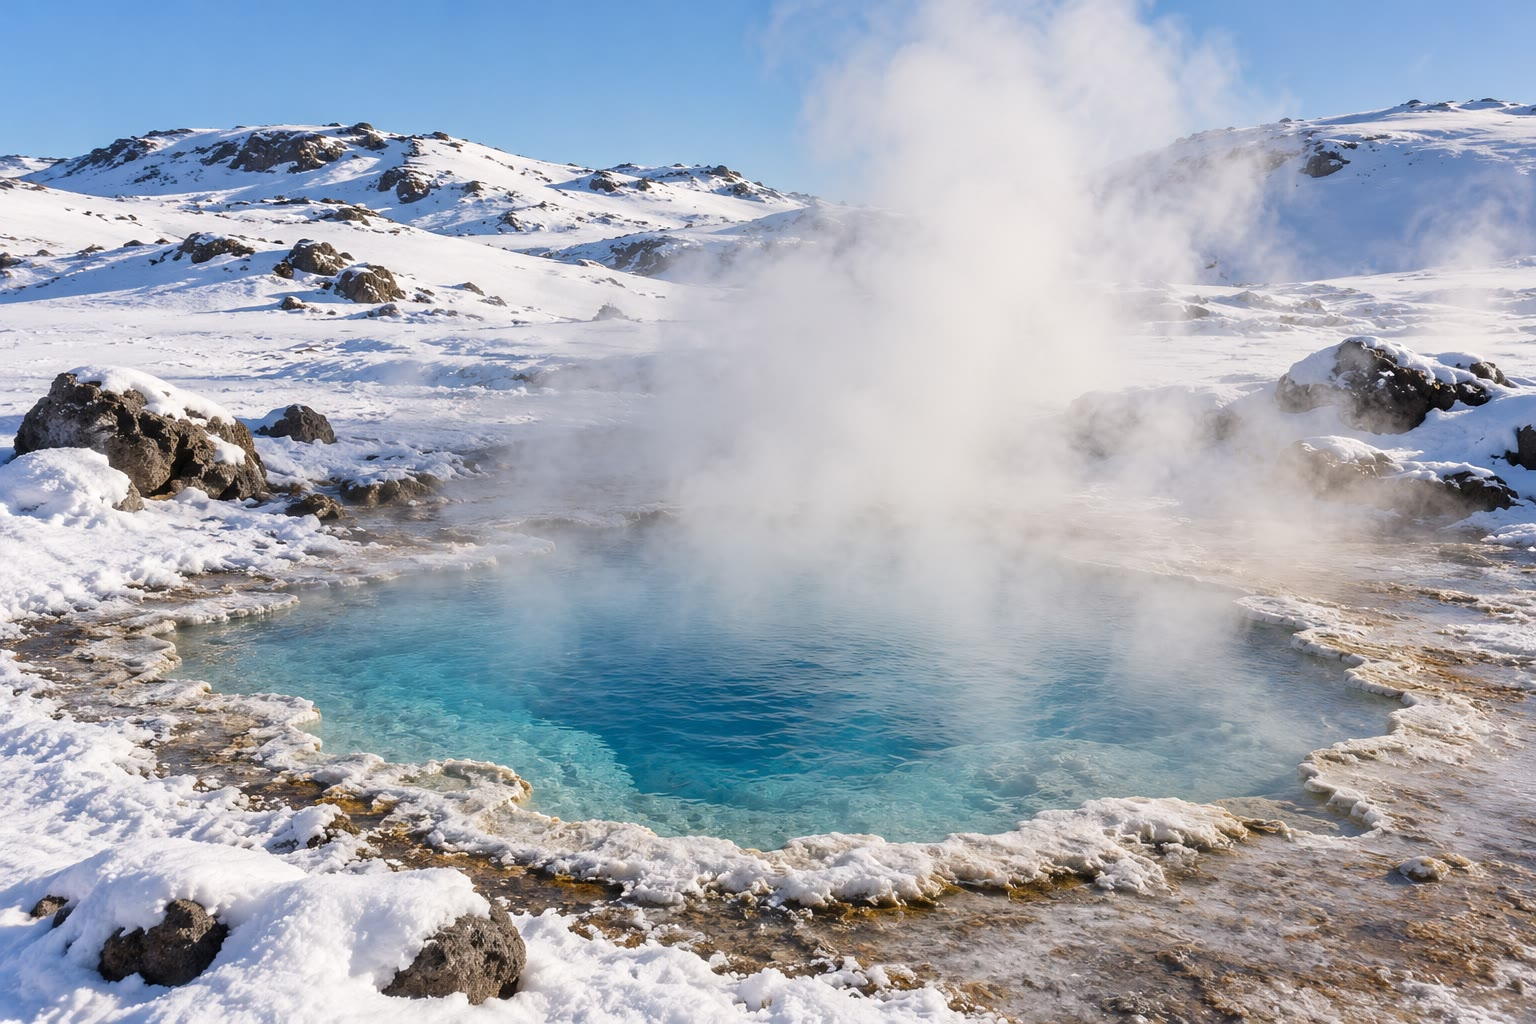
\includegraphics[width=0.6\linewidth]{images/book2/ai/g12-hot-spring-snow.jpg}

{\small Een warmwaterbron die dampt in een besneeuwd landschap: water dat diep
onder de grond is opgewarmd, komt terug naar het oppervlak. AI-illustratie.}
\end{omfigure}

\begin{omfigure}
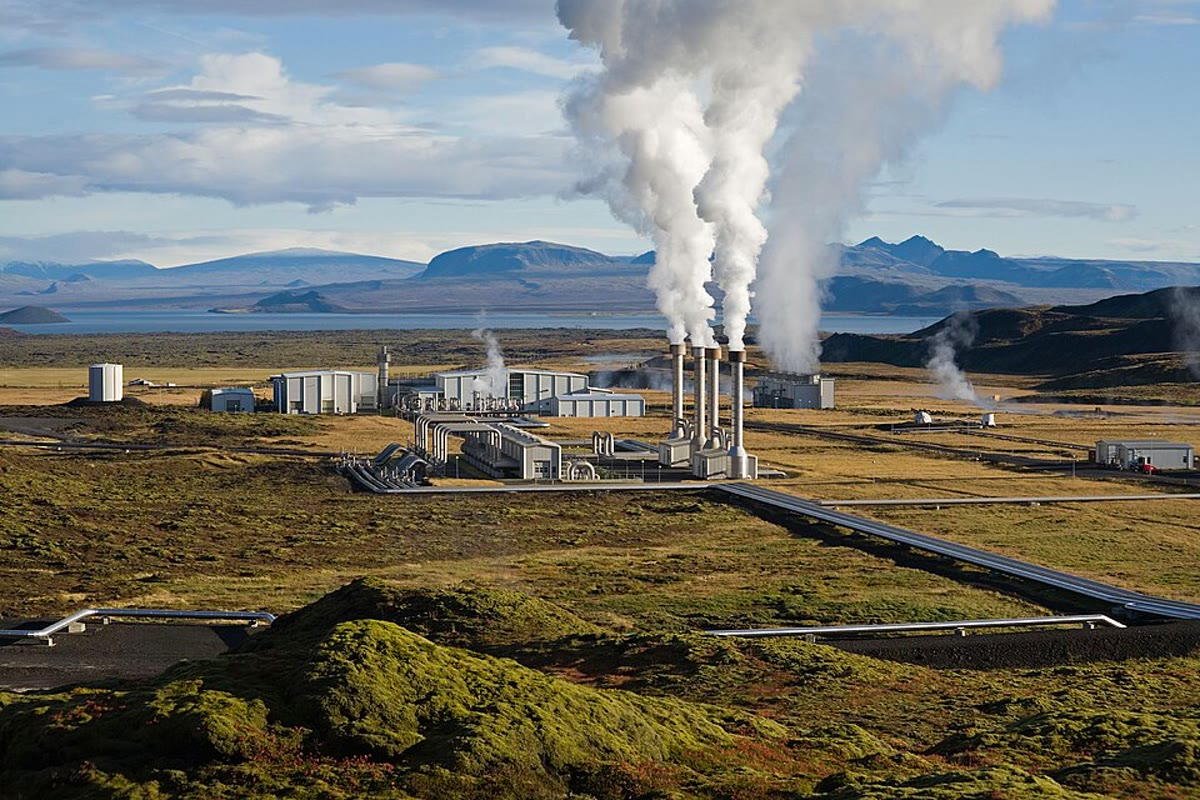
\includegraphics[width=0.66\linewidth]{images/book2/g12-nesjavellir-geothermal.jpg}

{\small De geothermische centrale van Nesjavellir, in het vulkanische gebied van de Hengill
in IJsland: tot \qty{120}{MW} elektriciteit en tot
\qty{300}{MW} warmte, meegevoerd door heet water. Foto Gretar
Ívarsson (publiek domein).}
\end{omfigure}
% ledger: photo:g12-nesjavellir, on:nesjavellir

Een geothermisch veld is op de schaal van een mensenleven niet onuitputtelijk. Bij The
Geysers, in Californië, onttrokken te veel putten stoom, sneller dan de
trage \omterm{def:g12:internal-heat:heat-flow}{warmtestroom} en de regen konden aanvullen: de druk van de stoom zakte
tot minder dan de helft van zijn piek, en meer dan \qty{40}{\percent} van de
capaciteit van de centrales ging verloren. Nu wordt er water teruggepompt in het
veld om de achteruitgang te vertragen.
% ledger: cpuc:geysers

\section{Oefeningen}

\begin{exercise}[$\star$]\label{exo:g12:internal-heat:1}
Geef het woord: (a) het vermogen dat het binnenste verlaat door elke vierkante meter
oppervlak; (b) de warmte die vrijkomt door het verval van radioactieve atomen in een
volume-eenheid gesteente; (c) het verlies van de warmte die sinds het ontstaan van de Aarde is opgeslagen;
(d) transport van warmte door de beweging van het materiaal zelf; (e) de inwendige
warmte van de Aarde die mensen gebruiken.
\end{exercise}

\begin{exercise}[$\star$]\label{exo:g12:internal-heat:2}
Reken om: (1) \qty{91.6}{mW/m^2} naar \unit{W/m^2}; (2) \qty{46.7}{TW} naar
watt; (3) \qty{29}{\celsius} per kilometer naar kelvin per meter.
\end{exercise}

\begin{exercise}[$\star$]\label{exo:g12:internal-heat:3}
Noem de vier isotopen die bijna alle radiogene warmte maken, en zeg
welke twee de detector KamLAND kan zien.
\end{exercise}

\begin{exercise}[$\star$]\label{exo:g12:internal-heat:4}
Bereken met $q = 490/\sqrt{t}$ de \omterm{def:g12:internal-heat:heat-flow}{warmtestroom} door oceaanbodem van 1, 4,
25 en 49 miljoen jaar oud.
\end{exercise}

\begin{exercise}[$\star$]\label{exo:g12:internal-heat:5}
Waarom wordt de \omterm{def:g12:internal-heat:heat-flow}{warmtestroom} in boorgaten gemeten en niet aan het oppervlak zelf?
Waarom moet je na het boren wachten voordat je meet?
\end{exercise}

\begin{exercise}[$\star\star$]\label{exo:g12:internal-heat:6}
In het KTB-boorgat had het gesteente op \qty{9.1}{km} ongeveer \qty{265}{\celsius}.
(1) Bereken de gemiddelde
gradiënt, met \qty{10}{\celsius} aan het oppervlak. (2) Welke \omterm{def:g12:internal-heat:heat-flow}{warmtestroom}
geeft die met een geleidingscoëfficiënt van \qty{2.72}{W/(m.K)}? (3) Vergelijk met het gemiddelde van de continenten.
\end{exercise}

\begin{exercise}[$\star\star$]\label{exo:g12:internal-heat:7}
De continenten beslaan \qty{2.073e14}{m^2} met een gemiddelde \omterm{def:g12:internal-heat:heat-flow}{warmtestroom} van
\qty{70.9}{mW/m^2}, de oceanen \qty{3.028e14}{m^2} met
\qty{105.4}{mW/m^2}. Bereken het vermogen dat elk verliest, het totaal, en het aandeel
dat door de oceaanbodem verloren gaat.
\end{exercise}

\begin{exercise}[$\star\star$]\label{exo:g12:internal-heat:8}
Een laag \omterm{def:g12:subduction-magmatism:granodiorite}{granodioriet} van \qty{8}{km} dik heeft een warmteproductie van
\qty{1.88}{\micro W/m^3}. (1) Welke \omterm{def:g12:internal-heat:heat-flow}{warmtestroom} produceert ze aan het oppervlak?
(2) Welk aandeel is dat van \qty{70.9}{mW/m^2}?
\end{exercise}

\begin{exercise}[$\star\star$]\label{exo:g12:internal-heat:9}
Op welke ouderdom verliest de oceaanbodem volgens $q = 490/\sqrt{t}$ evenveel warmte als het gemiddelde continent,
\qty{70.9}{mW/m^2}?
\end{exercise}

\begin{exercise}[$\star\star$]\label{exo:g12:internal-heat:10}
Hoeveel meer warmte maakte uranium-235 1.4 miljard jaar geleden vrij dan
vandaag? En kalium-40, 2.5 miljard jaar geleden?
\end{exercise}

\begin{exercise}[$\star\star$]\label{exo:g12:internal-heat:11}
Hoe lang doet warmte er met $t \approx L^2/\kappa$ en $\kappa = \qty{1e-6}{m^2/s}$ over
om door geleiding te doorkruisen: (1) een lavastroom van \qty{10}{m} dik;
(2) een \omterm{def:g11:lithosphere-asthenosphere:lithosphere}{lithosfeer} van \qty{100}{km} dik; (3) de mantel? Druk elk resultaat
uit in zinnige eenheden.
\end{exercise}

\begin{exercise}[$\star\star\star$]\label{exo:g12:internal-heat:12}
Vandaag maakt thorium-232 ongeveer \qty{10.4}{TW} vrij, uranium-238 \qty{9.6}{TW},
kalium-40 \qty{4.0}{TW} en uranium-235 \qty{0.42}{TW}. Bereken met de
halveringstijden van de figuur de warmte van
elk 3 miljard jaar geleden, het totaal, en het aandeel van de twee kortlevende
isotopen.
\end{exercise}

\begin{exercise}[$\star\star\star$]\label{exo:g12:internal-heat:13}
De centrale van Nesjavellir kan tot \qty{300}{MW} warmte leveren,
meegevoerd door ongeveer \qty{1640}{L} heet water per seconde. Met een soortelijke warmte
van \qty{4180}{J/(kg.K)} en een massa van \qty{1}{kg} per liter: met hoeveel
graden is dit water opgewarmd? Hoe groot is de oppervlakte van een gemiddeld continent
die \qty{300}{MW} warmte verliest?
\end{exercise}

\begin{exercise}[$\star\star\star$]\label{exo:g12:internal-heat:14}
Stel dat een plaat 100 miljoen jaar nodig heeft om van een rug tot een trog te gaan, en een
convectielus door de hele mantel ongeveer 200 miljoen jaar. (1)
Vergelijk deze tijden met de 260 miljard jaar van geleiding door de
mantel. (2) Waarom kan convectie warmte zoveel sneller vervoeren, hoewel de
mantel maar een paar centimeter per jaar beweegt?
\end{exercise}

\begin{exercise}[$\star\star\star$]\label{exo:g12:internal-heat:15}
Stel dat de kern ongeveer \qty{10}{TW} warmte aan de mantel verliest over
de \omterm{def:g11:seismic-structure:core}{kern-mantelgrens}, op \qty{2891}{km} diepte. (1) Welk aandeel van de
\omterm{def:g12:internal-heat:secular-cooling}{seculaire afkoeling}, \qty{22.3}{TW}, zou dat zijn? Waar komt de rest
vandaan? (2) Bereken de gemiddelde \omterm{def:g12:internal-heat:heat-flow}{warmtestroom} over de
\omterm{def:g11:seismic-structure:core}{kern-mantelgrens}, en vergelijk die met de gemiddelde \omterm{def:g12:internal-heat:heat-flow}{warmtestroom} aan het oppervlak,
\qty{91.6}{mW/m^2}. (3) Waarom kan de hete kern de basis van de mantel verwarmen
hoewel de mantel vast is?
\end{exercise}

\begin{problem}[{Weekendprobleem --- het warmtebudget van de Aarde}]
\label{pb:g12:internal-heat:1}
% ledger: b2dd10:continents, b2dd10:half-space, kamland11:geonu, dye12:isotopes, dye12:bse, b2vila:heat-production
% values (internal_heat.py): radiogenic 24.4 TW, secular 22.3 TW, share 0.523, K40 4.0, U235 0.42, U238 9.59
De \omterm{def:g12:internal-heat:heat-flow}{warmtestroom} van de Aarde is op meer dan 38\,000 plaatsen gemeten.
Gemiddeld verliezen de continenten \qty{70.9}{mW/m^2} over \qty{2.073e14}{m^2},
en de oceaanbodem \qty{105.4}{mW/m^2} over \qty{3.028e14}{m^2}.

\medskip
\noindent\textbf{Deel I --- Warmtestroom en oppervlakten.}
\begin{enumerate}
  \item Controleer dat de twee oppervlakten samen de oppervlakte van een bol met straal
        \qty{6371}{km} geven.
  \item Welk deel van het oppervlak is oceaanbodem?
  \item Waarom verliest de oceaanbodem meer warmte per vierkante meter dan de
        continenten?
  \item Bereken met $q = 490/\sqrt{t}$ de \omterm{def:g12:internal-heat:heat-flow}{warmtestroom} door oceaanbodem van
        4 miljoen jaar oud.
  \item Een boorgat in graniet (\qty{2.72}{W/(m.K)}) meet
        \qty{26}{\celsius} per kilometer. Ligt zijn \omterm{def:g12:internal-heat:heat-flow}{warmtestroom} boven of onder het
        continentale gemiddelde?
\end{enumerate}

\medskip
\noindent\textbf{Deel II --- Het totaal.}
\begin{enumerate}[resume]
  \item Bereken het vermogen dat door de continenten verloren gaat.
  \item Bereken het vermogen dat door de oceaanbodem verloren gaat.
  \item Tel ze op: de totale \omterm{def:g12:internal-heat:heat-flow}{warmtestroom} van de Aarde, in terawatt.
  \item Wat is de gemiddelde \omterm{def:g12:internal-heat:heat-flow}{warmtestroom} over het hele oppervlak?
  \item Als er onder elk continent \qty{10}{km} graniet (\qty{24.3}{mW/m^2}) lag,
        hoeveel terawatt zou dat produceren? Vergelijk met het
        vermogen dat door de continenten verloren gaat.
\end{enumerate}

\medskip
\noindent\textbf{Deel III --- Radiogene warmte.}
\begin{enumerate}[resume]
  \item KamLAND telt geoneutrino's van uranium-238 en thorium-232: samen
        maken ze ongeveer \qty{20.0}{TW} vrij, met \qty{3.9}{kg} thorium in
        de Aarde voor elke kilogram uranium. Een kilogram uranium maakt
        \qty{94.4}{\micro W} vrij via zijn uranium-238 en \qty{4.10}{\micro W}
        via zijn uranium-235; een kilogram thorium \qty{26.3}{\micro W}.
        Bereken de warmte van uranium-238, en daarna van uranium-235.
  \item Kalium-40 voegt er ongeveer \qty{4}{TW} aan toe. Bereken de totale radiogene warmte.
  \item Welke soort gesteente draagt het grootste deel van deze elementen, en waar ligt het?
  \item Was de radiogene warmte 3 miljard jaar geleden groter of kleiner? Waarom?
\end{enumerate}

\medskip
\noindent\textbf{Deel IV --- Seculaire afkoeling.}
\begin{enumerate}[resume]
  \item Welk vermogen wordt niet door radioactiviteit geleverd?
  \item Waar komt het vandaan?
  \item Bereken het aandeel van de \omterm{def:g12:internal-heat:heat-flow}{warmtestroom} dat door \omterm{def:g12:internal-heat:secular-cooling}{seculaire afkoeling} wordt geleverd.
  \item Modellen van de samenstelling van de Aarde geven een radiogene warmte van 11 tot
        \qty{38}{TW}.
        Tussen welke aandelen ligt het radiogene deel dan?
  \item Wat voert het grootste deel van deze warmte door de mantel?
  \item Vat samen: welk aandeel van het warmteverlies van de Aarde levert radioactiviteit
        vandaag?
\end{enumerate}
\end{problem}
